\chapter{Fundamentals of Algorithmic Efficiency}

\section{The Concept of Basic Operations}
We consider the most repeated operation of an algorithm to be its basic operation. By doing this, we can effectively mimic the working of the algorithm without much of the unnecessary complexity. 

For example, in bubble sort, we compare each element to the next element, even if we do not swap them. This implies that the basic operation of bubble sort is comparision.

This approach also helps us to approximate the time taken by an algorithm, by separating the execution and number of operations.

\[
    T(n) \approxeq c_{op} \cdot C(n)
\]
Where \mbox{\(T(n)\)} is the time taken for the execution of an algorithm for \mbox{\(n\)} inputs, \mbox{\(c_{op}\)} is the time required for the execution of the basic operation and \mbox{\(C(n)\)} is the number of basic operations for \mbox{\(n\)} inputs.

\section{The Three Notations}
There can by many algorithms designed around a problem statement. This, would necessitate a framework for comparision of algorithms. However, due to their virtue of being `methods', we have to eliminate the factor of `speed of operations' from such a comparision. For this, we are using three notations borrowed from mathematics.
\begin{gather*}
    \mathcal{O}\left( n \right)  \tag{Upper Bound}\\
    \Omega \left( n \right) \tag{Lower Bound}\\
    \Theta \left( n \right) \tag{Tight Bound}
\end{gather*}

It is important to stress here that these notations do not represent the best/worst/average cases. These are just mathematical notations, and a best/worst/average case can only be fixed for a particular input size.

Informally, we can think of \mbox{\(\mathcal{O}(n)\)} as representing the changes in performance of the algorithm with the worst cases at different sizes. Similarly, we can consider \mbox{\( \Omega \left( n \right)\)} as tracking the best case growth rate, and \mbox{\(\Theta \left( n \right)\)} doing the same for the average cases.



\begin{figure}
    \begin{center}
        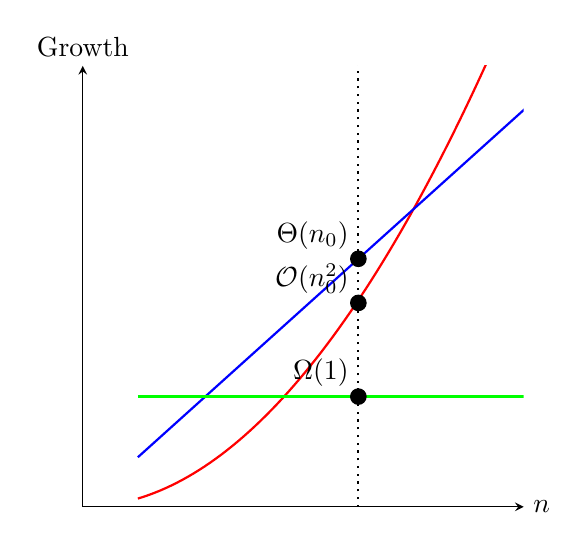
\begin{tikzpicture}[scale=1.4, >=stealth]
            % Axes
            \draw[->] (0,0) -- (4,0) node[right] {\(n\)};
            \draw[->] (0,0) -- (0,4) node[above] {Growth};

            % Functions with adjusted scaling
            \clip (0,0) rectangle (4,4); % Restrict everything inside the bounding box

            % Function plots
            \draw[thick, red] plot[domain=0.5:5.5, samples=100] (\x, {0.3*\x^2}) node[right] {\(\mathcal{O}(n^2)\)};
            \draw[thick, blue] plot[domain=0.5:5.5, samples=100] (\x, {0.9*\x}) node[right] {\(\Theta(n)\)};
            \draw[thick, green] plot[domain=0.5:5.5, samples=100] (\x, {1}) node[right] {\(\Omega(1)\)};

            % Vertical dotted line at n=n_0
            \draw[dotted, thick] (2.5,0) -- (2.5,5.5);

            % Corrected intersection points
            \filldraw (2.5,1) circle (2pt);
            \node[above left] at (2.5,1) {\(\Omega(1)\)};

            \filldraw (2.5,2.25) circle (2pt);
            \node[above left] at (2.5,2.25) {\(\Theta(n_0)\)};

            \filldraw (2.5,1.85) circle (2pt);  % Corrected height for O(n^2)
            \node[above left] at (2.5,1.85) {\(\mathcal{O}(n_0^2)\)};

            % Label for vertical line
            \node[below] at (2.5,0) {\(n_0\)};
        \end{tikzpicture}
    \end{center}
    \caption{Orders of Growth} \labelandindex{Orders of Growth}[fig:orderofgrowth]

\end{figure}

\Cref{fig:orderofgrowth} illustrates this point clearly. In this algorithm, the orders of growth are given by 
\[
    \mathcal{O}(n^2), \Theta(n) \text{ and } \Omega(1) \tag{These are notations}
\]
And for a particular choice of \mbox{\(n=n_0\)} 
\[
    \Omega(1) < \mathcal{O}(n_0^2) < \Theta(n_0)  \tag{These are cases}
\]
\textbf{Note:} This is not conventionally considered, as for the above case, \mbox{\(n_0 <1\)} which is meaningless in terms of computational inputs. But this is theoretically possible, and highlights the difference well.

\section{Formal Definitions}
\begin{definitiontcb}
    {\mbox{\(\mathcal{O}(g(n))\)}}{bigonotation}
    A function \mbox{\(f(n)\)} is said to be in \mbox{\(\mathcal{O}(g(n))\)} denoted as 
    \[
        f(n) \in \mathcal{O}(g(n))
    \]  
    If there exists some positive constant \mbox{\(c\)} and some non-negative integer \mbox{\(n_0\)} such that 
    \[
        f(n) \leq c \cdot g(n) \qquad \forall\, n\geq n_0
    \]
\end{definitiontcb}
\begin{definitiontcb}
    {\mbox{\(\Omega(g(n))\)}}{bigomeganotation}
    A function \mbox{\(f(n)\)} is said to be in \mbox{\(\Omega(g(n))\)} denoted as 
    \[
        f(n) \in \Omega(g(n))
    \]  
    If there exists some positive constant \mbox{\(c\)} and some non-negative integer \mbox{\(n_0\)} such that 
    \[
        f(n) \geq c \cdot g(n) \qquad \forall\, n\geq n_0
    \]
\end{definitiontcb}
\begin{definitiontcb}
    {\mbox{\(\Theta(g(n))\)}}{bigthetanotation}
    A function \mbox{\(f(n)\)} is said to be in \mbox{\(\Theta(g(n))\)} denoted as 
    \[
        f(n) \in \Theta(g(n))
    \]  
    If there exists some positive constants \mbox{\(c_1 \text{ and } c_2\)} and some non-negative integer \mbox{\(n_0\)} such that 
    \[
        c_2 \cdot g(n) \leq f(n) \leq c_1 \cdot g(n) \qquad \forall\, n\geq n_0
    \]
\end{definitiontcb}

\section{Worked Examples}
\begin{exampletcb}
    {Prove that \mbox{\(f(n) = 3n^2 + 2n + 7\)} belongs to \mbox{\(\mathcal{O}(n^3)\)}.}{bigonotation}
    From the question, we can infer that \mbox{\(g(n) = n^3\)}. According to \cref{defn:bigonotation}, we need to find constants \mbox{\(c\)} and \mbox{\(n_0\)} such that
    \begin{gather*}
        f(n) \leq c \cdot g(n) \qquad \forall\, n\geq n_0\\
        3n^2 + 2n + 7 \leq 1 \cdot n^3 \qquad \forall\, n\geq 3 \tag*{\mbox{\(n_0 = 3, c=1\)}}
    \end{gather*}
\end{exampletcb}

\begin{exampletcb}
    {Prove that \mbox{\(f(n) = 5n^3 - 4n + 8\)} belongs to \mbox{\(\Omega(n^3)\)}.}{bigomeganotation}
    From the question, we can infer that \mbox{\(g(n) = n^3\)}. According to \cref{defn:bigomeganotation}, we need to find constants \mbox{\(c\)} and \mbox{\(n_0\)} such that
    \begin{gather*}
        f(n) \geq c \cdot g(n) \qquad \forall\, n\geq n_0\\
        5n^3 - 4n + 8 \geq 1 \cdot n^3 \qquad \forall\, n\geq 2 \tag*{\mbox{\(n_0 = 2, c=1\)}}
    \end{gather*}
\end{exampletcb}

\begin{exampletcb}
    {Prove that \mbox{\(f(n) = 4n^2 + 10n + 20\)} belongs to \mbox{\(\Theta(n^2)\)}.}{bigthetanotation}
    From the question, we can infer that \mbox{\(g(n) = n^2\)}. According to \cref{defn:bigthetanotation}, we need to find constants \mbox{\(c_1, c_2\)} and \mbox{\(n_0\)} such that
    \begin{gather*}
        c_1 \cdot g(n) \leq f(n) \leq c_2 \cdot g(n) \qquad \forall\, n\geq n_0\\
        1 \cdot n^2 \leq 4n^2 + 10n + 20 \leq 5 \cdot n^2 \qquad \forall\, n\geq 5 \tag*{\mbox{\(n_0 = 5, c_1=1, c_2=5\)}}
    \end{gather*}
\end{exampletcb}

\section{Theorems for Asymptotic Notations}
Here are some useful theorems listed without proof for asymptotic notations.
\begin{theoremtcb}
    {Addition of \mbox{\(\mathcal{O}(g(n))\)}}{bigoadded}
    If \mbox{\(f_1(n) \in \mathcal{O}(g_1(n))\)} and \mbox{\(f_2(n) \in \mathcal{O}(g_2(n))\)}, then their sum satisfies
    \[
        f_1(n) + f_2(n) \in \mathcal{O}(\max(g_1(n), g_2(n))).
    \]
\end{theoremtcb}

\begin{theoremtcb}
    {Addition of \mbox{\(\Omega(g(n))\)}}{bigomegaadded}
    If \mbox{\(f_1(n) \in \Omega(g_1(n))\)} and \mbox{\(f_2(n) \in \Omega(g_2(n))\)}, then their sum satisfies
    \[
        f_1(n) + f_2(n) \in \Omega(\min(g_1(n), g_2(n))).
    \]
\end{theoremtcb}

\begin{theoremtcb}
    {Addition of \mbox{\(\Theta(g(n))\)}}{bigthetaadded}
    If \mbox{\(f_1(n) \in \Theta(g_1(n))\)} and \mbox{\(f_2(n) \in \Theta(g_2(n))\)}, then their sum satisfies
    \[
        f_1(n) + f_2(n) \in \Theta(\max(g_1(n), g_2(n))).
    \]
\end{theoremtcb}

